\documentclass[border=10pt]{standalone}
\usepackage[svgnames]{xcolor}
\usepackage{amsmath}
\usepackage{pgfplots}
\pgfplotsset{compat=newest}
\usepackage[sfdefault]{FiraSans}
\usepackage{FiraMono}
\renewcommand*\familydefault{\sfdefault}
\begin{document}
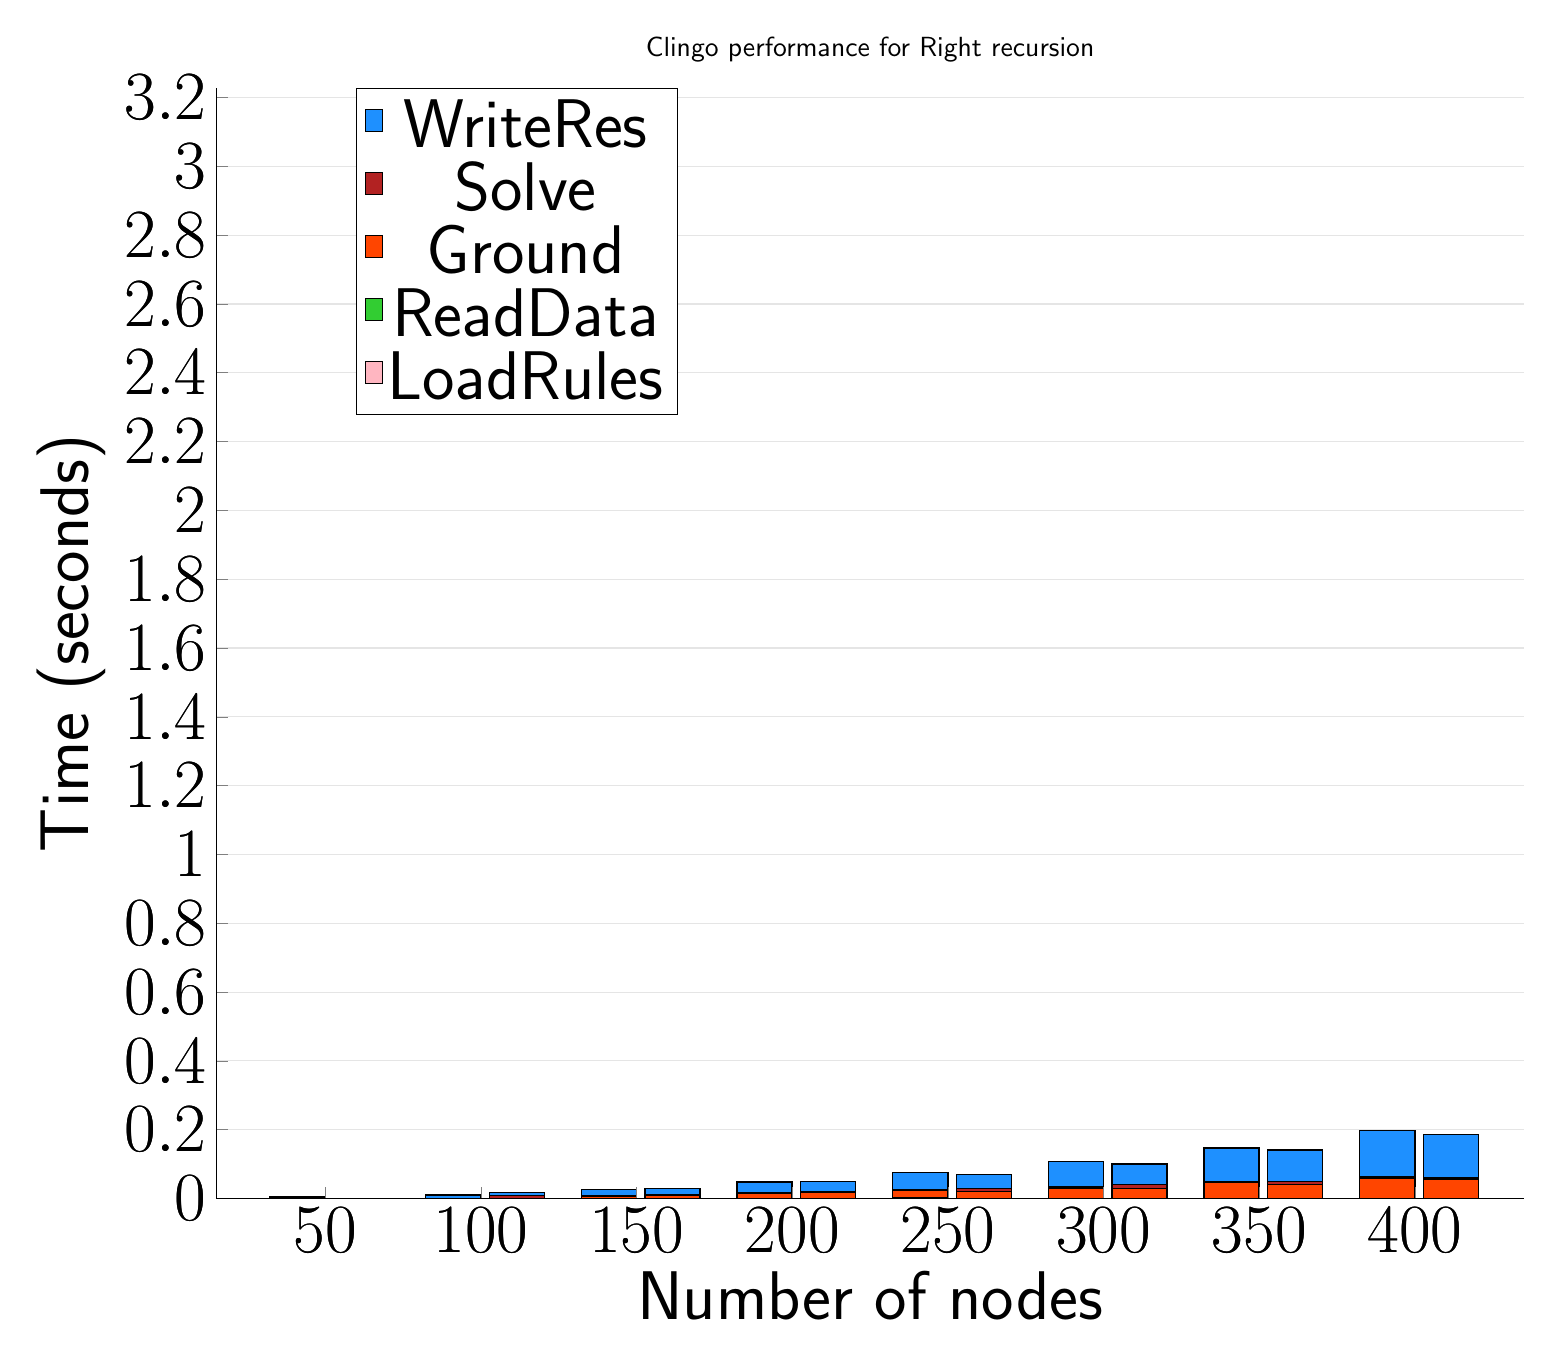
\begin{tikzpicture}
\begin{axis}[
   ybar stacked,
   title={Clingo performance for Right recursion},
   bar shift=-10pt,
   width=1.5\textwidth,
   bar width=0.7cm,
   ymajorgrids, tick align=inside,
   major grid style={draw=gray!20},
   xtick=data,
   ymin=0, ymax=3.2279999971389772,
   axis x line*=bottom,
   axis y line*=left,
   enlarge x limits=0.1,
   legend style={
       at={(0.23, 1)},
       anchor=north,
       legend columns=1,
       font=\Huge,
   },
   ylabel={Time (seconds)},
   xlabel={Number of nodes},
   label style={font=\Huge},
   tick label style={font=\Huge},
]
\addlegendimage{fill=DodgerBlue, draw=black, line width=0.2pt}
\addlegendentry{WriteRes}
\addlegendimage{fill=FireBrick, draw=black, line width=0.2pt}
\addlegendentry{Solve}
\addlegendimage{fill=OrangeRed, draw=black, line width=0.2pt}
\addlegendentry{Ground}
\addlegendimage{fill=LimeGreen, draw=black, line width=0.2pt}
\addlegendentry{ReadData}
\addlegendimage{fill=LightPink, draw=black, line width=0.2pt}
\addlegendentry{LoadRules}
\addplot +[fill=LightPink, draw=black, line width=0.5pt] coordinates {
    (50, 0.0)
    (100, 0.0)
    (150, 0.0)
    (200, 0.0)
    (250, 0.0009999990463256836)
    (300, 0.0)
    (350, 0.0)
    (400, 0.0)
};
\addplot +[fill=LimeGreen, draw=black, line width=0.5pt] coordinates {
    (50, 0.0)
    (100, 0.0)
    (150, 0.0)
    (200, 0.0)
    (250, 0.0009999990463256836)
    (300, 0.0)
    (350, 0.0009999990463256836)
    (400, 0.0)
};
\addplot +[fill=OrangeRed, draw=black, line width=0.5pt] coordinates {
    (50, 0.0029999971389770507)
    (100, 0.0)
    (150, 0.008000016212463379)
    (200, 0.015999984741210938)
    (250, 0.02200000286102295)
    (300, 0.03100001811981201)
    (350, 0.04499998092651367)
    (400, 0.05999996662139893)
};
\addplot +[fill=FireBrick, draw=black, line width=0.5pt] coordinates {
    (50, 0.0)
    (100, 0.0)
    (150, 0.0009999990463256836)
    (200, 0.0019999980926513673)
    (250, 0.0019999980926513673)
    (300, 0.0029999971389770507)
    (350, 0.0039999961853027345)
    (400, 0.0029999971389770507)
};
\addplot +[fill=DodgerBlue, draw=black, line width=0.5pt] coordinates {
    (50, 0.0029999971389770507)
    (100, 0.009999990463256836)
    (150, 0.016999983787536622)
    (200, 0.030000019073486327)
    (250, 0.05000004768371582)
    (300, 0.07299997806549072)
    (350, 0.09699997901916504)
    (400, 0.1340000867843628)
};
\end{axis}
\begin{axis}[
   ybar stacked,
   bar shift=13pt,
   width=1.5\textwidth,
   bar width=0.7cm,
   ymajorgrids, tick align=inside,
   major grid style={draw=none},
   xtick=data,
   ymin=0, ymax=3.2279999971389772,
   axis x line*=none,
   axis y line*=none,
   enlarge x limits=0.1,
   label style={font=\Huge},
   tick label style={font=\Huge},
]
\addplot +[fill=LightPink, draw=black, line width=0.5pt] coordinates {
    (50, 0.0)
    (100, 0.0)
    (150, 0.0)
    (200, 0.0)
    (250, 0.0)
    (300, 0.0)
    (350, 0.0)
    (400, 0.0)
};
\addplot +[fill=LimeGreen, draw=black, line width=0.5pt] coordinates {
    (50, 0.0)
    (100, 0.0)
    (150, 0.0)
    (200, 0.0)
    (250, 0.0)
    (300, 0.0)
    (350, 0.0)
    (400, 0.0)
};
\addplot +[fill=OrangeRed, draw=black, line width=0.5pt] coordinates {
    (50, 0.0)
    (100, 0.0009999999999999998)
    (150, 0.009999999999999997)
    (200, 0.018999999999999996)
    (250, 0.019999999999999997)
    (300, 0.030000000000000006)
    (350, 0.04099999999999999)
    (400, 0.05600000000000001)
};
\addplot +[fill=FireBrick, draw=black, line width=0.5pt] coordinates {
    (50, 0.0)
    (100, 0.007999999999999997)
    (150, 0.0)
    (200, 0.0010000000000000002)
    (250, 0.010000000000000004)
    (300, 0.009999999999999995)
    (350, 0.009000000000000008)
    (400, 0.003999999999999998)
};
\addplot +[fill=DodgerBlue, draw=black, line width=0.5pt] coordinates {
    (50, 0.0)
    (100, 0.008999999999999998)
    (150, 0.020000000000000007)
    (200, 0.029000000000000005)
    (250, 0.039999999999999994)
    (300, 0.06000000000000001)
    (350, 0.09099999999999998)
    (400, 0.12599999999999997)
};
\end{axis}
\end{tikzpicture}

\end{document}
